\documentclass{article}

% --------------- PAQUETES ---------------
\usepackage[utf8]{inputenc}
\usepackage[spanish]{babel}
\usepackage{amsmath, amssymb}
\usepackage{physics}
\usepackage{siunitx}
\usepackage{xcolor}
\usepackage{tcolorbox}
\usepackage{cancel}
\usepackage{multicol}
\usepackage[
    top=2.5cm,
    bottom=2.5cm,
    left=3.3cm,
    right=3.3cm
]{geometry}
\usepackage{tikz}
\usetikzlibrary{angles, quotes}
\usepackage{float}
\usepackage{hyperref}  


% --------------- COLORES PERSONALIZADOS ---------------
\definecolor{sectionColor}{HTML}{2240f0}
\definecolor{definicionColor}{HTML}{2240f0}
\definecolor{titleColor}{HTML}{ff0000}
\definecolor{exerciceColor}{HTML}{00d5ff}

% --------------- COMANDOS PERSONALIZADOS ---------------
\newcommand{\newsection}[1]{
    \section{\centering \color{sectionColor} \bl{#1}}
}

\newcommand{\newsubsection}[1]{
    \subsection{\color{sectionColor} #1}
}

\newcommand{\newtitle}[1]{
    \vspace{0.5cm}
    \noindent{\large \color{titleColor} \textbf{#1}}\\[0.2cm]
}

\newcommand{\newex}[1]{
    \vspace{0.5cm}
    \noindent{\large \color{exerciceColor} \textbf{#1}}\\[0.2cm]
}

\newcommand{\bl}[1]{\textbf{#1}}


\newtcolorbox{definicionbox}{
    colback=white,      % fondo blanco
    colframe=blue,     % borde negro
    boxrule=2pt,      % grosor del borde
    arc=0pt,            % sin esquinas redondeadas
    left=10pt, right=8pt, top=8pt, bottom=10pt, % margen interno
}

\newcommand{\definicion}[1]{%
    \begin{definicionbox}
        #1
    \end{definicionbox}
}

% --------------- ENCABEZADO ---------------
\title{Apunte Física 1}
\author{Luca Di Bene}
\date{\today}

% --------------- DOCUMENTO ---------------
\begin{document}

    \maketitle
    \tableofcontents
    \newpage

% ------------------- SECCIÓN 1 -------------------
    \newsection{Unidades, Cantidades Físicas y Vectores}

    % ----------------- NUEVA SUBSECCIÓN -----------------

    \newsubsection{La Física}

    \par La Física es una \bl{ciencia experimental} que busca explicar fenómenos naturales a través de la observación y la experimentación. Los físicos formulan teorías mediante \bl{modelos ideales, leyes y principios físicos}. Estas teorías se desarrollan con creatividad, pruebas y observaciones, como hizo Galileo al investigar la caída de los cuerpos.

    \newtitle{Resolución de problemas}

    \par Resolver problemas permite aplicar conceptos. El proceso incluye:

    \begin{enumerate}
        \item \underline{Identificar conceptos}: Elegir qué principios físicos son relevantes.
        \item \underline{Plantear el problema}: Traducirlo a ecuaciones.
        \item \underline{Ejecutar la solución}: Sustituir valores y hacer cálculos.
        \item \underline{Evaluar la respuesta}: Verificar si tiene sentido físico.
    \end{enumerate} 

    \begin{multicols}{2}

    \begin{center}
    \begin{minipage}[t]{0.60\textwidth}
    \newtitle{Modelos idealizados}
        \smallskip

        \par En física, simplificamos los sistemas complejos creando \bl{modelos idealizados} que omiten detalles irrelevantes. Estos modelos son válidos dentro de ciertos límites, como el modelo de caída libre de Galileo que omite la resistencia del aire.
        \par La física describe el mundo mediante \bl{modelos matemáticos}, que permiten hacer predicciones razonables sobre el comportamiento de los sistemas.

    \end{minipage}

    \hfill
    \columnbreak
    
    \begin{minipage}[t]{0.35\textwidth}

        \bigskip
        \par Para simplificar el análisis de a) una pelota de béisbol lanzada al aire, usamos b) un modelo idealizado.
        \smallskip
        \par a) Una pelota real lanzada al aire.
        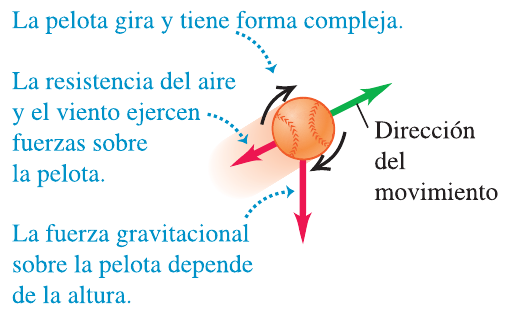
\includegraphics[width=\linewidth]{img/1.1-1.png}

        \par b) Un modelo idealizado de una pelota real lanzada al aire.
        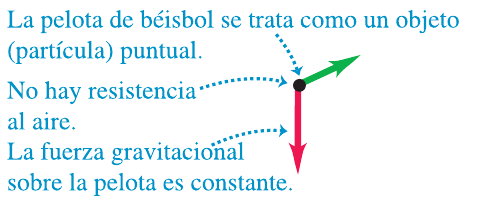
\includegraphics[width=\linewidth]{img/1.1-2.png}

    \end{minipage}
    \end{center}

    \end{multicols}

    % ----------------- NUEVA SUBSECCIÓN -----------------

    \newsubsection{Mediciones, magnitudes y unidades}

    \newtitle{Magnitudes físicas y unidades}

    \par Las \bl{magnitudes físicas} son propiedades medibles como masa, longitud o tiempo. El \bl{Sistema Internacional (SI)} define unidades básicas:

    \begin{itemize}
        \item \bl{Longitud}: metro (\bl{m})
        \item \bl{Masa}: kilogramo (\bl{kg})
        \item \bl{Tiempo}: segundo (\bl{s})
    \end{itemize}

    \par Las unidades derivadas (como velocidad o energía) se forman combinando unidades básicas.

    \newtitle{Conversión de unidades}

    \begin{enumerate}
        \item \underline{Identificar}: qué unidades hay que convertir.
        \item \underline{Plantear/Ejecutar}: usar factores de conversión.
        \item \underline{Evaluar}: comprobar que tenga sentido.
    \end{enumerate}

    \[
        3\cancel{\text{min}} \times \frac{60s}{1\cancel{\text{min}}} = 180s
    \]

    \newtitle{Incertidumbre}

    \par Toda medición tiene \bl{incertidumbre}, que refleja el límite del instrumento. Se expresa como:

    \[
        \text{valor medido} \pm \text{error}
    \]

% ------------------- NUEVA SUBSECCIÓN -------------------
    \newsubsection{Vectores y Suma de Vectores}

    \newtitle{Cantidades escalares y vectoriales}

    \par En física, algunas cantidades pueden ser descritas solo con un número y una unidad (\bl{escalares}), como el tiempo, la masa o la temperatura. Otras, en cambio, requieren una dirección además de una magnitud (\bl{vectores}). La velocidad y la fuerza son ejemplos típicos: no basta con saber cuánto valen, también es esencial saber \bl{hacia dónde} actúan o se mueven.
    \par Un vector se representa con una \bl{flecha}. La \bl{longitud} indica la magnitud y la \bl{orientación} muestra su dirección. Por convención, los vectores se nombran con letras negritas y con una \bl{flecha arriba}, como \(\vec{A}\), para diferenciarlos de los escalares.

    \begin{figure}[H]
        \centering
        \shorthandoff{>}
        \begin{tikzpicture}[scale=2]
            \draw[->] (0,0) -- (2,1) node[midway, above] {$\vec{A}$};
        \end{tikzpicture}
    \end{figure}

    \definicion{
        \centering
        \par \underline{Magnitud}: A o \(\lvert \vec{A} \rvert\) indican cuánto mide \(\vec{A}\), sin dirección.
        }

    \begin{multicols}{2}
        \centering

        \begin{minipage}[t]{0.6\textwidth}

            \par Dos vectores son \bl{iguales} si tienen la misma \bl{magnitud} y \bl{dirección}, aunque estén ubicados en lugares diferentes.

        \end{minipage}
        \hfill
        \columnbreak
        \begin{minipage}[t]{0.3\textwidth}

            \begin{figure}[H]
                \centering
                \shorthandoff{>}
                \begin{tikzpicture}[scale=1.2]
                    \draw[->, blue] (0,0) -- (1,1) node[midway, above] {$\vec{A}$};
                    \draw[->, red] (1,0) -- (2,1) node[midway, above] {$\vec{B}$};
                \end{tikzpicture}
                \shorthandon{>}
            \end{figure}

        \end{minipage}
        
    \end{multicols}

    \begin{multicols}{2}
        \centering

        \begin{minipage}[t]{0.6\textwidth}

            \par Un vector \bl{opuesto} tiene igual magnitud pero direción contraria, lo llamamos el negativo del vector original.

        \end{minipage}
        \hfill
        \columnbreak
        \begin{minipage}[t]{0.3\textwidth}

            \begin{figure}[H]
                \centering
                \shorthandoff{>}
                \begin{tikzpicture}[scale=1.2]
                    \draw[->, blue] (0,0) -- (1,1) node[midway, above] {$\vec{A}$};
                    \draw[->, red] (2,1) -- (1,0) node[midway, below, right] {$\vec{B}=-\vec{A}$};
                \end{tikzpicture}
                \shorthandon{>}
            \end{figure}

        \end{minipage}
        
    \end{multicols}

    \par \underline{Suma de vectores}: Para sumar vectores gráficamente, se usa el metodo "\bl{cola con punta}": se coloca el origen del segundo vector en el extremo del primero.
    \begin{figure}[H]
        \centering
        \shorthandoff{>}
        \begin{tikzpicture}[scale=1]
            \draw[->, gray] (0,0) -- (3,1) node[midway, below] {$\vec{A}$};
            \draw[->, gray] (3,1) -- (2,3) node[midway,right] {$\vec{B}$};
            \draw[->, blue] (0,0) -- (2,3) node[midway, above, left] {$\vec{A}+\vec{B}$};
        \end{tikzpicture}
        \shorthandon{>}
    \end{figure}

    \par No importa el orden en que sumes los vectores, siempre da el mismo resultado.
    \[ \vec{A}+\vec{B}=\vec{B}+\vec{A} \]

    \par \underline{Resta de vectores}: Restar vectores significa sumar el \bl{opuesto}. Si queremos calcular \(\vec{A}-\vec{B}\), lo que realmente hacemos es sumar \(\vec{A}\) con el negativo de \(\vec{B}\).
    \[ \vec{A}-\vec{B}=\vec{A}+(-\vec{B}) \]

    % ---------------- NUEVA SUBSECCIÓN ----------------

    \newsubsection{Componentes de vectores}

    \par Cuando sumamos vectores, muchas veces es más fácil descomponerlos en \bl{componentes} sobre un sistema de ejes perpendiculares.
    \par Un vector \(\vec{A}\) puede descomponerse en dos vectores: uno paralelo al eje x (\(\vec{A}_x\)) y otro paralelo al eje y (\(\vec{A}_y\)). La suma de estos dos vectores da como resultado el vector original: \(\vec{A}=\vec{A}_x+\vec{A}_y\).

    \begin{figure}[H]
        \centering
        \shorthandoff{>}
        \begin{tikzpicture}[scale=1.2]
            \draw[->, black] (0,0) -- (3,0) node[below] {$x$};
            \draw[->, black] (0,0) -- (0,3) node[left] {$y$};

            \draw[->, blue] (0,0) -- (1,2) node[midway, above, left] {$\vec{A}$};
            \draw[->, red] (0,0) -- (1,0) node[midway, below] {$\vec{A}_x$};
            \draw[->, green] (0,0) -- (0,2) node[midway, above, left] {$\vec{A}_y$};
            \draw[-, dashed, gray] (1,0) -- (1,2);
            \draw[-, dashed, gray] (0,2) -- (1,2);

            % angle
            \draw[->, black] (0.5,0) .. controls (0.5,0.4) and (0.3,0.5) ..  (0.25,0.5) node[midway, above, right] {$\theta$};

        \end{tikzpicture}
        \shorthandon{>}
    \end{figure}

    \par Podemos calcular la magnitud de las componentes de $\vec{A}$ si conocemos la magnitud A y su dirección. Describimos la direccion de un vector como el angulo $\theta$ formado por le eje x positivo con el vector en sentido anti horario. Entonces por definición de trigonométricas:
    \[ \lvert \vec{A}_x \rvert = \lvert \vec{A} \rvert \cos \theta \]
    \[ \lvert \vec{A}_y \rvert = \lvert \vec{A} \rvert \sin \theta \]

% ------------------- SECCIÓN 2 -------------------

\newsection{Leyes del movimiento de Newton}

\par En los dos capítulos anteriores estudiamos la cinemática, el lenguaje para describir el movimiento. Ahora estamos en condiciones de pensar en qué hace que los cuerpos se muevan como lo hacen.

\par En este capítulo usaremos dos conceptos nuevos, la fuerza y la masa, para analizar los principios de la dinámica, los cuales están establecidos en solo tres leyes que fueron claramente enunciadas por Sir Isaac Newton:

\begin{itemize}
    \item Primera ley (ley de la inercia): Si la fuerza neta sobre un cuerpo es cero, su movimiento no cambia.
    \item Segunda ley: Relaciona la fuerza con la aceleración cuando la fuerza neta no es cero.
    \item Tercera ley: Es una relación entre las fuerzas que ejercen dos cuerpos que interactúan entre sí.
\end{itemize}

\par Las leyes de Newton no son producto de deducciones matemáticas, sino una síntesis que los físicos han descubierto al realizar un sinnúmero de experimentos con cuerpos en movimiento.

    % ---------------- NUEVA SUBSECCIÓN ----------------

    \newsubsection{Fuerza e interacciones}

        \par En la vida cotidiana hablamos de fuerza como un empujón o un tirón. En física, una fuerza se define mejor como una interacción entre dos cuerpos o entre un cuerpo y su entorno. Esta interacción tiene dirección y magnitud, por lo que se representa como un vector.

    \newtitle{Fuerzas de contacto}

        \par Son fuerzas que requieren interacción directa entre cuerpos. Se distinguen principalmente tres tipos:

        \begin{itemize}
            \item \underline{Fuerza normal}: Es la fuerza ejercida por una superficie sobre un objeto en contacto con ella. Siempre actúa perpendicular a la superficie.
            \item \underline{Fuerza de fricción}: También es ejercida por una superficie, pero actúa paralela a ella y en dirección opuesta al movimiento relativo entre el objeto y la superficie.
            \item \underline{Fuerza de tensión}: Es la fuerza transmitida por cuerdas, cables o cordeles estirados. Actúa a lo largo del cordel y en la dirección de la tracción, como cuando se tira de una cuerda.
        \end{itemize}

        \begin{multicols}{3}
            \centering
            \begin{figure}[H]
                \centering
                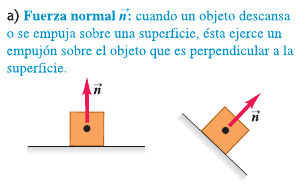
\includegraphics[scale=0.6]{img/2.1-1.png}
                \caption{Fuerza normal}
                \label{fig:Fuerza normal}
            \end{figure}

            \columnbreak

            \begin{figure}[H]
                \centering
                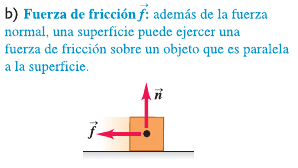
\includegraphics[scale=0.6]{img/2.1-2.png}
                \caption{Fuerza de fricción}
                \label{fig:Fuerza de fricción}
            \end{figure}

            \columnbreak

            \begin{figure}[H]
                \centering
                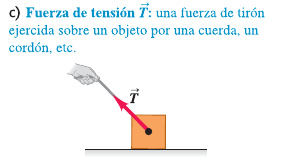
\includegraphics[scale=0.6]{img/2.1-3.png}
                \caption{Fuerza de tensión}
                \label{fig:Fuerza de tension}
            \end{figure}

        \end{multicols}

    \newtitle{Fuerzas a distancia}
        \par Estás actuar sin contacto física Ejemplos comunes son la gravedad, el magnetismo y las fuerzas eléctricas. La fuerza gravitatoria que la tierra ejerce sobre un objetto se llama \bl{peso}.
        \begin{figure}[H]
            \centering
            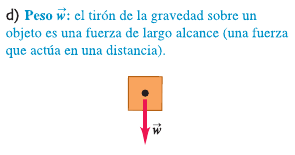
\includegraphics[scale=0.8]{img/2.1-4.png}
            \caption{Fuerza a distancia}
            \label{fig:Fuerza a distancia}
        \end{figure}

    \newtitle{Medición de fuerzas}

        \par La magnitud de una fuerza se mide en "newtons", que se abrevia N. (Daremos una definición precisa del newton más adelante) Un instrumento tipico para medirla es la \bl{balanza de resorte} que aprovecha la relación entre estiramento de un resorte y la fuerza aplicada.

    \newtitle{Superposición de fuerzas}

        \par Cuando varias fuerzas actúan sobre un cuerpo, su efecto combinado es igual al de una única fuerza resultante obtenida mediante la suma vectorial de todas ellas. Esto se conoce como el Principio de superposición. La fuerza neta o resultante total sobre un cuerpo es, la suma vectorial de todas las fuerzas que actúan sobre él. Se denota:
        
        \[\vec{R} = \sum \vec{F}\]

        \par Cada fuerza puede descomponerse en componentes vectoriales, entonces la fuerza neta tambien:

        \[\vec{R_x} = \sum \vec{F_x} \quad , \quad \vec{R_y} = \sum \vec{F_y}\]

    \newsubsection{Primera ley de Newton}

    \definicion{
        \par \color{blue}\underline{\bl{Primera ley}}\color{black}: Todo cuerpo persevera en su estado de reposo o movimiento uniforme y rectilíneo a no ser que sea obligado a cambiar su estado por fuerzas impresas sobre él. 
    }

    \par En esta ley se introduce el concerto de \bl{inercia}, que es la resistencia de un cuerpo a cambiar su estado de movimiento.
    \par Esta ley rompe con la idea aristotélica de que se necesita una fu constante para mantener el movimiento. Newton muestra que en r lo que se necesita es una fuerza para cambiar el movimiento.
    \par Si empujás una caja y después dejas de hacerlo, eventualmente se detiene. No porque "el movimiento se gasta", sino porque existen fuerzas Como la fricción y el rozamiento con el aire que actúan en sentido Contrario al movimiento y Provocan que se frene.

    \newtitle{Marcos de referencia inerciales}

    \par Un \bl{marco de referencia} es un sistema desde el cual se observa y describe el movimiento de los cuerpos.
    \par Un \bl{marco de referencia inercial} es aquel en el cual se cumple la Primera Ley de Newton, es decir que si un objeto cambia su Velocidad, entonces desde el marco se ve una fuerza actuando.

    \newsubsection{Segunda ley de Newton}

    \par Podemos ver que existe una relación proporcional entre la fuerza y la aceleración. Si empujamos una caja con una fuerza neta constante, la caja tendra una acelarión constante igual a $a=\vec{a}$.
    \par Si utilizamos una balanza de resorte Para aplicar una fuerza $\vec{F_1}$ obtenemos una aceleración $\vec{a}$, para $2\vec{F_1}$, obtenemos $2\vec{a}$ y para $\frac{1}{2}\vec{F_1}$ $\frac{1}{2}\vec{a}$. Muchos experimentos semejantes muestran que para un cuerpo dado, la magnitud de la aceleración es directamente propor-cional a la magnitud de la fuerza neta que actúa sobre él.

    \newtitle{Masa y fuerza}

   \par Nuestros resultados indican que para un cuerpo dado, el cociente $\left\lvert \Sigma \vec{F}\right\rvert $ entre $\left\lvert \vec{a} \right\rvert $ es constante. Llamamos a este cocient \bl{masa inercial} del cuerpo y la denotamos con \bl{m}. Es decir,

    \[ m = \frac{\lvert \Sigma \vec{F}\rvert }{\lvert \vec{a} \rvert } \quad,\quad
    \lvert \Sigma \vec{F} \rvert = m \lvert \vec{a} \rvert \quad o \quad
    \lvert \vec{a} \rvert = \frac{\lvert \Sigma \vec{F}\rvert }{m}\]

    \par La ultima de las ecuaciones indica que cuanto mayor sea su masa, más se "resiste" un cuerpo a ser acelerado.
    \par La unidad de masa en el SI es el kilogramo. Podemos usar este Kilogramo para definir el newton:

    \definicion{
        \par Un Newton es la cantidad de fuerza neta que proporciona una aceleración de 1 metro por segundo al cuadrado a un cuerpo con masa de 1 Kilograma.
    }

    \par Por la forma en que definimos el newton, está relacionado con las unidades de masa, longitud y tiempo.

    \[ 1 \text{N} = 1 \text{kg} \cdot \text{m/s}^2 \]

    \begin{table}[H]
        \centering
        \begin{tabular}{|c|c|c|c|}
            \hline
            Sistema de unidades & Fuerza & Masa & Aceleración \\
            \hline
            SI & Newton(N) & Kg & $m/s^2$ \\
            \hline
            cgs & dina(din) & g & $cm/s^2$ \\
            \hline
            Imperial & libra(lb) & slug & $ft/s^2$ \\
            \hline
        \end{tabular}
    \end{table}

    \newtitle{Enunciado de la segunda ley de Newton}

    \definicion{
        \par \color{blue}\underline{\bl{Segunda ley}}\color{black}: si una fuerza externa neta actúa sobre un Cuerpo, éste se acelera. La dirección de aceleración es la mis ma que la dirección de la fuerza neta. El vector de fuerza neta es igual a la masa del cuerpo multiplicada por su aceleración. En símbolos: 

        \[\Sigma \vec{F} = m \vec{a}\]
    }

    \par La segunda ley de Newton es una ley fundamental de la naturaleza, la relación básica entre fuerza y movimiento, Casa todo el resto del capítulo, y todo el que sigue, se dedica a aprender a aplicar este principio en diversas situaciones.

    \newtitle{Uso de la segunda ley de Newton}

    \par Hay al menos cuatro aspectos de la segundo ley de Newton que Merecen atención especial:

    \begin{enumerate}
        \item \bl{Forma de uso}: La segunda lev de Newton es una ecuación Vectorial, Pero normalmente se usa descompuesta por componentes:
        \[\Sigma \vec{F_x} = m \vec{a_x} \quad , \quad \Sigma \vec{F_y} = m \vec{a_y}\]

        \item \bl{Fuerzas externes}: La ley se refiere únicamente a Fuerzas externas es decir, ejercidas sobre el cuerpo desde otros cuerpos o el entorno. Un cuerpo no puede moverse por una fuerza que el mismo genera.
        \item \bl{Masa constante}: Estas ecuaciones solo son válidas si las masa no cambia. En casos donde la masa varía (cohete que pierda combustible) se necesita un tratamiento especial.
        \item \bl{Marcos de referencia inenciales}: La ley solo se aplica en marcos de referencia inerciales. No vale en marcos acelerados, como dentro de un auto que arranca.
    \end{enumerate}

    \newsubsection{Masa y Peso}

    \begin{multicols}{2}
        \begin{minipage}[t]{0.7\textwidth}
            \par Es común usar incorrecta e indistintamente los términos \bl{masa} y \bl{peso} en las conversaciones cotidianas. Es absolutamente indispensable entender claramente las diferencias entre estas dos cantidades físicas.

            \par La \bl{masa} Caracteriza las Propiedades inerciales de un cuerpo. A mayor masa, se necesitará más fuerza Para causar una aceleración dada.

            \par El \bl{peso}, en cambio, es una fuerza ejercida sobre un cuerpo por la atracción de la Tierra.

            \par Para entender la relación entre masa y peso, note que un cuerpo en caída libre tiene una aceleración igual a gy, Por la segunda ley de Newton, una fuerza produce esa aceleración. Si un cuerpo de masam cae con una aceleración $\vec{g}$ con $ \lvert \vec{g} \rvert = 9.8 \text{m/s}^2 $, entonces: $\vec{w} = m \vec{g}$
        \end{minipage}

        \columnbreak

        \begin{minipage}[t]{0.7\textwidth}
            \begin{figure}[H]
                \centering
                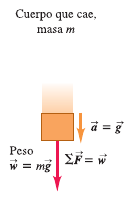
\includegraphics[scale=1]{img/2.4-1.png}
            \end{figure}
        \end{minipage}
    \end{multicols}

    \newtitle{Variación de g con la ubicación}

    \par En la tierra se usa $g \approx 9,80 m/s^2$, Pero varía entre $9,78$ y $9,82 m/s^2$. Esa variación se debe a la forma de la tierra y su rotación. El peso cambia con g, Pero la masa no.

    \newtitle{Medición de masa y peso}

    \par En la práctica, se mide la masa de un cuerpo midiendo su peso y Comparándolo con un estandar. Por la ecuación $w=mg$, si dos cuerpos tienen el mismo peso en el mismo lugar, entonces tienen la misma masa.

    \newsubsection{Tercera ley de Newton}

    \par No podemos tirar de una perilla sin que ésta tire de nosotros. Al Patear un balón de fútbol, la fuerza hacia adelante que el rie ejerce sobre él lo lanza en su trayectoria, pero sentimos la fuerza que el balón ejerce sobre el pie.
    \par Los experimentos muestran que, al interactuar dos cuerpos, las fuer-zas que ejercen mutuamente son iguales en magnitud y opuestas en dire-ceión. Ésta es la tercera ley de Newton.

    \definicion{
        \par \color{blue}\underline{\bl{Tercera ley}}\color{black}: si el cuerpo A eserce una fuerza sobre el cuerpo. B ("\text{acción}"), entonces, B ejerce una fuerza sobre A ("\text{reacción}"). Estas dos fuerzas tienen la misma magnitud Pero dirección opuesta, y actúan sobre diferentes cuerpos.
        \[\vec{F}_{AB} = - \vec{F}_{BA}\]
    }

    \begin{figure}[H]
        \centering
        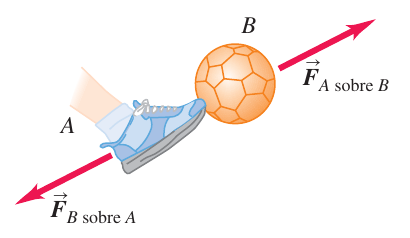
\includegraphics[scale=0.8]{img/2.5-1.png}
    \end{figure}

    \par Expresando en palabras, en la tercera ley de Newton, "acción" y "reacción" son las dos fuerzas opuestas, y Podemos llamarlas \bl{Par acción-reacción}.

    \newsubsection{Diagramas de cuerpo libre}

    \par En esta sección mencionaremos algunas ideas y técnicas que Pueden usarse en cualquier problema en que intervengan las leves de Newton.

    \begin{enumerate}
        \item Las leves de Newton se aplican a un cuerpo específico. Siempre tenés que definir que cuerpo vas a analizar.
        \item En la sumatoria de fuerzas F, solo se incluyen las fuerzas que actúan sobre el cuerpo, no las que el cuerpo ejerce sobre otros. Si analizás a una persona caminando, incluís la fuerzas del suelo sobre la persona, no la que la persona ejerce sobre el suelo.
        \item Un diagrama de cuerpo libre muestra el cuerpo aislado con todas las fuerzas externas que actúan sobre el, sin incluir fuerzas que el cuerpo ejerce sobre otros.
    \end{enumerate}

    \begin{figure}[H]
        \centering
        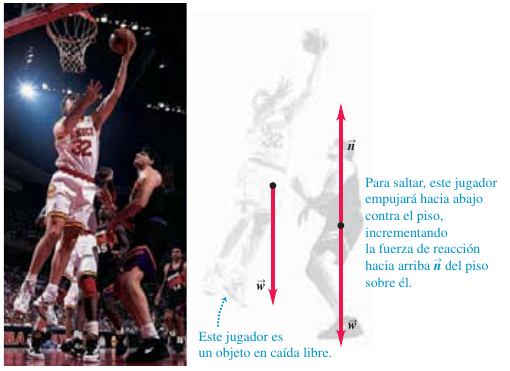
\includegraphics[scale=0.7]{img/2.6-1.png}
    \end{figure}

\newsection{Aplicación de las leyes de Newton}

\par Este capítulo se enfoca en \bl{aplicar las leyes de Newton} a distintos tipos de situaciones reales, como un velero deslizándose sobre hielo, un trineo bajando una colina y un avión dando una vuelta cerrada. A pesar de que las \bl{leyes de Newton} son simples en su formulación, resolver problemas concretos requiere una buena dosis de análisis y técnica.

    \newsubsection{Empleo de la primera ley de Newton: Partículas en equilibrio}

    \par El principio físico fundamental es la primera ley de Newton: si una partícula está en reposo o se mueve con velocidad constante en un marco de referencia inercial, la fuerza neta que actúa sobre ella, es decir, la suma vectorial de todas las fuerzas que actúan sobre ella debe ser cero:

    \definicion{
        \centering
        \par $\Sigma \vec{F} = 0 \quad$ (partícula en equilibrio, forma vectorial)
    }

    \par Esta sección trata sobre el uso de la primera ley de Newton para resolver problemas de cuerpos en equilibrio. Quizás algunos de los problemas parezcan complicados; no obstante, lo importante es recordar que todos los problemas que implican partículas en equilibrio se resuelven igual.

    \newex{Ejercicio 1. Equilibrio unidimensional: Tensión en una cuerda sin masa}

    \par Una gimnasta de masa $m_G = 50.0 kg$ se cuelga del extremo inferior de una cuerda colgante. El extremo superior está fijo al techo de un gimnasio. Suponga que la masa de la cuerda es despreciable.
    \begin{enumerate}
        \item ¿Cuánto pesa la gimnasta?
        \item ¿Qué fuerza (magnitud y dirección) ejerce la cuerda sobre ella?
        \item ¿Qué tensión hay en la parte superior de la cuerda?
    \end{enumerate}
    
    \newex{Solución 1.}

    \par Primero identificamos que la gimnasta y la cuerda, ambos estan en equilibrio. Tenemos como incognita el peso de la gimnasta $w_G$. La cuerda tira de la gimnasta con una fuerza $T_{CG}$ y la gimnasta tira de la cuerda con una fuerza $T_{GC}$. El techo ejerce otra fuerza sobre la cuerda, $T_{TC}$, que provoca que la cuerda y la gimnasta esten en equilibrio.

    \begin{figure}[H]
        \centering
        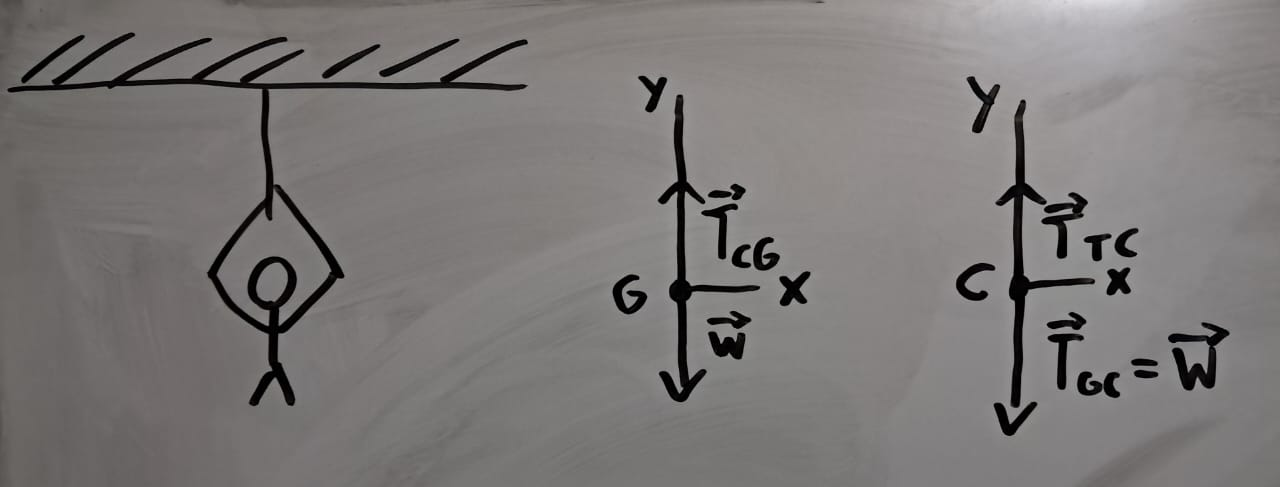
\includegraphics[width=\textwidth]{img/3.1-1.png}
    \end{figure}

    \par El primer digrama representa la situación en si. El segundo diagrama representa las fuerzas que actúan sobre la gimnasta. El tercer diagrama representa las fuerzas que actúan sobre la cuerda.

    \quad

    \par Para calcular el peso de la gimnasta ($\vec{w}$), usaremos la ecuación de la gravedad, derivada de la segunda ley de Newton:

    \[ \lvert \vec{w} \rvert = m \cdot 9.8 \text{m/s}^2 \]
    \[ w_G = 50 \text{kg} \cdot 9.8 \text{m/s}^2 \]
    \[ w_G = 490 \text{N} \]

    \begin{center}
        \par \bl{El peso de la gimnasta es de 490 Newtons}.
    \end{center}

    \par Entonce la magnitud de la fuerza que ejerce la cuerda sobre la gimnasta es: $T_{CG} = 490 \text{N}$. Y su dirección es contraria a la del peso de la gimnasta.

    \par Por el par acción-reacción, existe la fuerza $\vec{T}_{GC} = - \vec{T}_{CG} = \vec{w}$, entonces la gimnasta tira de la cuerda con una fuerza de 490 Newtons con una dirección que apunta hacia abajo. Entonces la fuerza $\vec{T}_{TC}$ es igual en magnitud a $\vec{T}_{GC}$ pero con dirección opuesta, es decir, $\vec{T}_{TC} = - \vec{T}_{GC}$.

    \quad

    \par La \bl{tensión de la cuerda} es de $T_{TC} = 490 \text{N}$ en la parte superior de la cuerda y de $T_{CG} = 490 \text{N}$ en la parte inferior de la cuerda.

    \newtitle{Empleo de la segunda ley de Newton: Dinámica de partículas}

    \par Ahora podemos analizar problemas de dinámica, donde aplicamos la segunda ley de Newton a cuerpos sobre los cuales la fuerza neta no es cero, de manera que los cuerpos no están en equilibrio sino que tienen aceleración.

    \definicion{
        \centering
        \( \Sigma \vec{F} = m \vec{a} \)
    }

    \newex{Ejercicio 2. Movimiento rectilíneo con una fuerza constante}

    \par Un velero para hielo descansa en una superficie horizontal sin fricción (figura 5.7a). Sopla un viento constante (en la dirección de los patines del trineo), de modo que 4.0 s después de soltarse el velero adquiere una velocidad de 6.0 m>s (unos 22 km/h o 13 mi/h). ¿Qué fuerza constante $F_w$ ejerce el viento sobre el velero? La masa total del velero más el tripulante es de 200 kg.

    \newex{Solución 2.}

    \par Identificamos las variables que se nos dan:

    \begin{itemize}
        \item $m = 200 \text{kg}$
        \item $v(0s) = 0.0 \text{m/s}$
        \item $v(4s) = 22.0 \text{km/h} = 6.1 \text{m/s}$
    \end{itemize}

    \par Para calcular la fuerza usaremos la segunda ley de Newton: $\Sigma \vec{F} = m \vec{a}$. Pero primero debemos calcular la aceleración. Como tenemos una velocidad incial y otra 4s despues podemos utilizar:
    \[ a = \frac{v_1 - v_0}{t_1 - t_0} \]

    \[ a = \frac{6.1 \text{m/s} - 0.0 \text{m/s}}{4.0 \text{s}} = 1.525 \text{m/s}^2 \]

    \par Por lo tanto, la fuerza constante que ejerce el viento sobre el velero es de $F_w = 200 \text{kg} \cdot 1.525 \text{m/s}^2 = 305 \text{N}$

    \newtitle{Peso aparente e ingravidez aparente}

    \par Cuando un pasajero de masa m viaja en un elevador con aceleración ay , una báscula da como peso aparente del pasajero:

    \[ w = m \cdot (g + a_y) \]

    \par Cuando el elevador está acelerando hacia arriba, $a_y$ es positiva y $n$ es mayor que el peso del pasajero $w = mg$. Si el elevador acelera hacia abajo, ay es negativa y n es menor que el peso. Si el pasajero no sabe que el elevador está acelerando, sentirá que su peso cambia y, de hecho, la báscula lo indica. El caso extremo sucede cuando el elevador tiene una aceleración hacia abajo $a_y = -g$, es decir, cuando está en caída libre. En este caso, $n = 0$ y el pasajero siente que no tiene peso.

    \newex{Ejercicio 3. Aceleración cuesta abajo}

    \par Un trineo cargado de estudiantes en vacaciones (peso total $w$) se desliza hacia abajo por una larga cuesta nevada. La pendiente tiene un ángulo constante $\alpha$, y el trineo está tan bien encerado que la fricción es despreciable. ¿Qué aceleración tiene el trineo?

    \par ...

    \newtitle{Fuerzas de fricción}

    

\end{document}